\documentclass{school-22.211-notes}
\date{April 25, 2012}

\begin{document}
\maketitle

\lecture{Point Kinetics Without Feedback}
\topic{Physics of Delayed Neutrons}
\textbf{Prompt neutrons}: more than 99\% of all neutrons are emitted in $<10^{-10}$s after the fission (prompt neutron lifetime in a PWR is about $2 \times 10^{-5}$ sec). Example: A reactor was operated at 1W, a control rod was moved to produce an excess reactivity of $0.0005 \Delta k$, what would the power be 1s later? 
\begin{align}
P(t) &= P_0 (1.0005)^{t/(2\times 10^{-5})} = 1 W (1.0005)^{1/(2\times 10^{-5})} = 70,000 MW 
\end{align}
The above calculation means that this reactor would be virtually impossible to control! Fortunately, delayed netrons exist and the reactor time constant depend on more than just prompt neutron lifetime. 

\textbf{Delayed neutrons}:
\begin{enumerate}
\item Measurement: delayed neutrons can be measured by counting neutrons emission after a pulsed irradiation of a pure U235 foil. Burst measurement represents the amount of prompt neutrons; saturated measurement represents the total amount of neutrons. 
\item Emission: delayed neutrons are emitted through the decay of fission products, of which Br-37 is a dominant FP that emits delayed neutrons. 
\item Delayed yields depend on fissioning species and neutron energy (keep in mind that U238 produce 4\% delayed neutron per fission, more than U235's 1.7\% delayed neutron per fission, making U238 a very important isotope when it comes to delayed neutrons). 
  \begin{itemize}
  \item Absolute yield: number of delayed neutrons per fission; unit: 1/fission. 
  \item Relative yield: absolute yield of an isotope divided by total absolute yield by all isotopes; 
  \item Delayed neutron fraction: absolute yield divided by $\bar{\nu}$. Number of delayed neutrons devided by number of total fission neutrons. 
  \end{itemize}
  \begin{table}[ht]
    \centering
    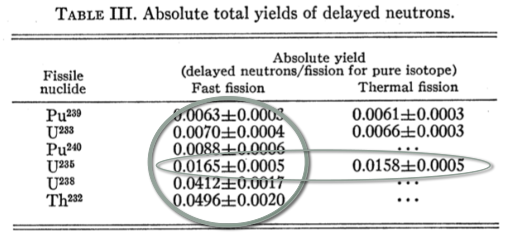
\includegraphics[width=4in]{images/pke/abs-yield.png}
    \caption{Absolute Total Yields of Delayed Neutrons} \label{abs-yield} 
  \end{table}
\item Modern trend: makes the 6-group to 8-group, and each group has a fixed decay constants (the one that dominants in the group, that is, largest half-life). This way, all isotopes have the same half-life for the same group; but different isotopes would still have different delayed neutron fraction. Remember the terms circled in blue.  
\item Delayed neutrons spectrum vs. energy: average prompt neutron emission energy is 2 MeV; average delayed neutron emission energy is 0.4 MeV. Both spectrum comes out to be Maxwellian, except the delayed one is shifted as in Fig.~\ref{fission-spec}. Delayed neutron comes out in the thermal energy range, which makes them more likely to fission. 
  \begin{figure}[ht]
    \centering
    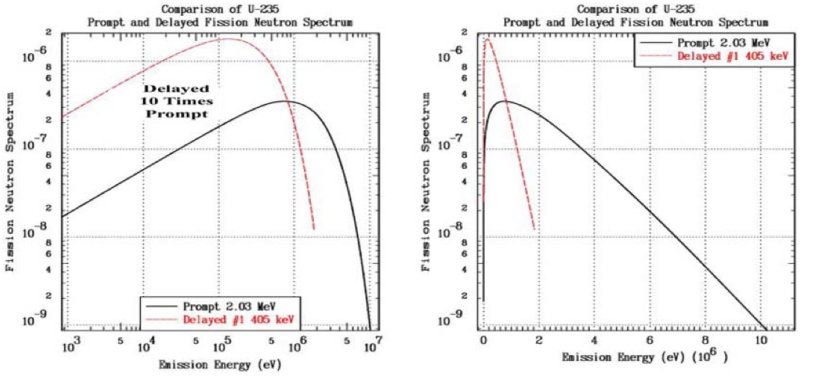
\includegraphics[width=4in]{images/pke/fission-spec.png}
    \caption{Prompt and Delayed Fission Neutron Spectrum} \label{fission-spec} 
  \end{figure}
\item Delayed energy group: neutron spectra have similar shapes for all delayed groups. However different energy groups have different mean energies. 
  \begin{figure}[ht]
    \centering
    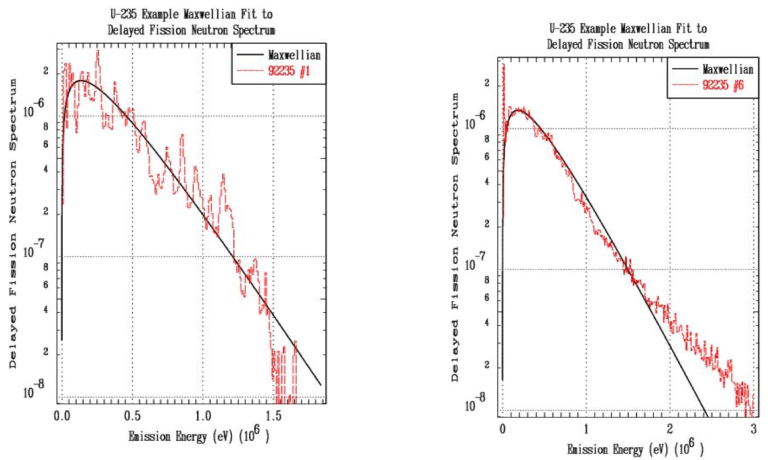
\includegraphics[width=4in]{images/pke/delayed-fission-spec.png}
    \caption{Delayed Fission Neutron Spectrum} \label{delayed-fission-spec} 
  \end{figure}
\item Take-away message: delayed neutron spectra vary only slightly for different fissioning nuclides; but the spectra depends significantly on the delayed neutron group. 
\end{enumerate}

\clearpage
\topic{Derivation of PKE}
In steady-state transport or diffusion equation, we do not treat delayed neutrons directly. But the fission emission spectrum must be properly weighted with prompt and delayed contributions. Notice one issue is, we need fission rates to get $\chi$, and we need $\chi$ to get fission rates, so the real way to solve the balance equation is to iterate, though this is not how it is done normally.
\begin{enumerate}
\item We start from the diffusion equation: \hi{The steady-state diffusion equation}\footnote{Know this for the final}: 
\small
\begin{align}
& - \divergence D(\vecr, E, t) \gradient \phi(\vecr, E, t) + \Sigma_t (\vecr, E, t) \phi(\vecr, E, t) = \int_0^{\infty} \Sigma_s (\vecr, E'\to E, t) \phi(\vecr, E', t) \dE' \\
&+ \Sum_j \chi_T^j (E) \int_0^{\infty} \nu \Sigma_p^j (\vecr, E', t) \phi(\vecr, E', t) \dE' + Q(\vecr, E, t) 
\end{align}
\normalsize

\item \hi{The time-dependent neutron diffusion equation}: where $\beta^j = \Sum_i \beta_i^j$ is the delayed fission fraction (0.66\% for instance), 
  \begin{align}
    \ppt \left[ \frac{1}{v} \phi(\vecr, E, t) \right] &= \divergence D(\vecr, E, t) \gradient \phi(\vecr, E, t) - \Sigma_t (\vecr, E, t) \phi(\vecr, E, t) 
\notag \\
    & + \int_0^{\infty} \Sigma_s (\vecr, E'\to E, t) \phi(\vecr, E', t) \dE'\notag \\
    &+ \Sum_j \chi_p^j (E) (1-\beta^j) \int_0^{\infty} \nu \Sigma_f^j (\vecr, E', t) \phi(\vecr, E', t) \dE'\notag \\
    &+ \Sum_i \chi_d^i (E) \lambda_i C_i (\vecr, t) + Q(\vecr, E, t)\\
    \ppt C_i (\vecr, t) &= \Sum_j \beta_i^j \int_0^{\infty} \nu \Sigma_p^j (\vecr, E', t) \phi(\vecr, E', t) \dE'  - \lambda_i C_i (\vecr, t) 
  \end{align}

\item Assume that flux can be separated into a space/energy term and a time-dependent term: $\phi(\vecr, E, t) = S(\vecr, E) T(t)$ ($S(\vecr, E)$ is the Shape function,  $T(t)$ is the amplitude function). Plug it into the above expressions. 
  \begin{align}
    \ppt \left[ \frac{1}{v} S(\vecr, E) T(t) \right] &= 
    \Bigg\{ \divergence D(\vecr, E, t) \gradient S(\vecr, E) - \Sigma_t (\vecr, E, t) S(\vecr, E)   \notag \\
    & + \int_0^{\infty} \Sigma_s (\vecr, E'\to E, t) S(\vecr, E') \dE'   \notag \\
    &+ \Sum_j \left( \chi_p^j (E) (1-\beta^j) + \Sum_i \chi_d^i (E) \beta_i^j \right) \int_0^{\infty} \nu \Sigma_f^j (\vecr, E', t) S(\vecr, E') \dE'   \notag \\
    &- \Sum_j \chi_p^j (E) \beta^j \int_0^{\infty} \nu \Sigma_f^j (\vecr, E', t) S(\vecr, E') \dE' \Bigg\} T(t)  \notag \\
    &+ \Sum_i \chi_d^i (E) \lambda_i C_i (\vecr, t) + Q(\vecr, E, t)   \\
    \ppt C_i (\vecr, t) &= \left\{ \Sum_j \beta_i^j \int_0^{\infty} \nu \Sigma_p^j (\vecr, E', t) S(\vecr, E') \dE' \right\} T(t) - \lambda_i C_i (\vecr, t) 
  \end{align}


\clearpage
\item Integrate over all space and energy and normalize to $\int \dE \int \dr \frac{1}{v} S(\vecr, E) = 1.0$, 
  \begin{align}
    \ddt \left[ T(t) \right] &= 
    \int \dE \int \dr \Bigg\{ \divergence D(\vecr, E, t) \gradient S(\vecr, E) - \Sigma_t (\vecr, E, t) S(\vecr, E)   \notag \\
    & + \int_0^{\infty} \Sigma_s (\vecr, E'\to E, t) S(\vecr, E') \dE'   \notag \\
    &+ \Sum_j \left( \chi_p^j (E) (1-\beta^j) + \Sum_i \chi_d^i (E) \beta_i^j \right) \int_0^{\infty} \nu \Sigma_f^j (\vecr, E', t) S(\vecr, E') \dE'   \notag \\
    &- \Sum_j \chi_p^j (E) \beta^j \int_0^{\infty} \nu \Sigma_f^j (\vecr, E', t) S(\vecr, E') \dE' \Bigg\} T(t)  \notag \\
    &+ \int \dE \int \dr \left[ \Sum_i \chi_d^i (E) \lambda_i C_i (\vecr, t) + Q(\vecr, E, t)\right]   
  \end{align}
  \begin{align}
    \ddt \left[ \int \dE \int \dr C_i (\vecr, t) \right] &= \int \dE \int \dr \left\{ \Sum_j \beta_i^j \int_0^{\infty} \nu \Sigma_p^j (\vecr, E', t) S(\vecr, E') \dE' \right\} T(t) \notag \\
    &- \lambda_i \int \dE \int \dr C_i (\vecr, t) 
  \end{align}


\item We define a set of terms to simplify the expression. For simplicity concern, we omit the dependency on the following terms. $D(\vecr, E, t), \Sigma_t (\vecr, E, t), \Sigma_f(\vecr, E, t),  S(\vecr, E), \chi(E)$. 
\begin{enumerate}
\item Reactivity $\rho(t)$, where the top is the diffusion equation, and the bottom is fission rate if all the neutrons show up instatenously. 
\scriptsize
\begin{align}
\rho (t) &= \frac{\int \bsp \dE \! \int \bsp \dr \Bigg\{ \!\divergence \! D  \gradient S  - \! \Sigma_t S  + \! \int \bsp \Sigma_s (\vecr \!, E' \bsp \to \bsp E, t) S \! \dE'   
    + \! \Sum_j \left( \! \chi_p^j (E) (1 \! - \! \beta^j) +  \! \Sum_i \chi_d^i (E) \beta_i^j \! \right) \! \int \bsp \nu \Sigma_f^j  S \dE'  }{\int \bsp \dE \int \bsp \dr \Sum_j \left( \chi_p^j (E) (1-\beta^j) + \Sum_i \chi_d^i (E) \beta_i^j \right) \int \bsp \nu \Sigma_f^j S \dE'} 
\end{align}
\normalsize
\eqn{ \Aboxed{ \rho(t) &= \frac{\keff - 1.0}{\keff}  } }


\item The delayed neutron fraction (notice although this is called delayed neutron fraction, there is $\chi_p^j(E)$ term in it), 
\begin{align}
\beta_i (t) &= \frac{\int \bsp \dE \int \bsp \dr \left[ \Sum_j \chi_d^j (E) \beta^j \int_0^{\infty} \nu \Sigma_f^j (\vecr, E', t) S(\vecr, E') \dE' \right] }{\int \bsp \dE \int \bsp \dr \Sum_j \left( \chi_p^j (E) (1-\beta^j) + \Sum_i \chi_d^i (E) \beta_i^j \right) \int \bsp \nu \Sigma_f^j S \dE'} 
\end{align}

\item Prompt neutron lifetime, 
\begin{align}
\Lambda (t) &= \frac{\int \bsp \dE \int \bsp  \dr \left[ \frac{1}{v} S(\vecr, E) \right] }{\int \bsp \dE \int \bsp \dr \Sum_j \left( \chi_p^j (E) (1-\beta^j) + \Sum_i \chi_d^i (E) \beta_i^j \right) \int \bsp \nu \Sigma_f^j S \dE'} 
\end{align}
\eqn{ \Aboxed{ \Lambda(t) &\approx \frac{1}{v \nu \Sigma_f} \xrightarrow{\mathrm{criticality}} \frac{1}{v \Sigma_a} } }
The prompt neutron life $\Gamma \sim 1/v$ of shape divided by almost-instantenous-fission-rate. 
\item The $i$-th precursor, 
  \eqn{ C_i (t) = \int \dE \int \dr C_i (\vecr, t) }
\item The total eternal source, 
  \eqn{ Q(t) = \int \dE \int \dr Q (\vecr, t) }
\end{enumerate}

\item Using the freshly defined terms, we get the classic \hi{point kinetics equations (PKE)},
\eqn{ \Aboxed{ \ddt T(t) &= \frac{\rho(t) - \Sum_i \beta_i (t) }{\Lambda (t)} T(t) + \Sum_i \lambda_i C_i (t) + Q(t) } }
\eqn{ \Aboxed{ \ddt C_i (t) &= \frac{\beta_i (t)}{\Lambda (t)} T(t) - \lambda_i C_i (t) }  }
Remember that the above classic PKEs are obtained using \uline{assumptions}: 
\begin{itemize}
\item No external source.
\item Constant $\beta_i, \lambda_i$. 
\item The approximation $\phi(\vecr, E, t) = S(\vecr, E) T(t)$, which is not always valid. 
\item There is no feedback (e.g., the reactor is operating at low enough flux, no feedback, coefficients are independent of solution), if $\rho(t)$ is known, one can solve for reactor power as a function of time.
\end{itemize}

\item For a steady state solution at power level $T_0$, we know, 
  \begin{align}
    \ddt C_i (0) &= 0  &\Rightarrow  C_i (0) &= \frac{\beta_i}{\Lambda \lambda_i} T_0  \notag \\
    \ddt T(0) &= 0  &\Rightarrow \rho(0) &= 0  \label{in-hour}
  \end{align}

\item \hi{The matrix form of the 1st order ODE} is (assuming three precursor groups, can be easily extend for more precursor groups),  
\begin{align}
N &= \left[ \begin{array}{c} T \\ C_1 \\ C_2 \\ C_3 \end{array} \right]  
& \ddt N(t) &= \left[ \begin{array}{cccc} 
\frac{\rho(t) - \beta}{\Lambda} & \lambda_1 & \lambda_2 & \lambda_3 \\
\frac{\beta_1}{\Lambda} & - \lambda_1 & & \\
\frac{\beta_2}{\Lambda} & & -\lambda_2 & \\
\frac{\beta_3}{\Lambda} & & & -\lambda_3 \end{array} \right] 
\left[ N(t) \right] 
\end{align}

%\begin{figure}[ht]
%  \centering
%  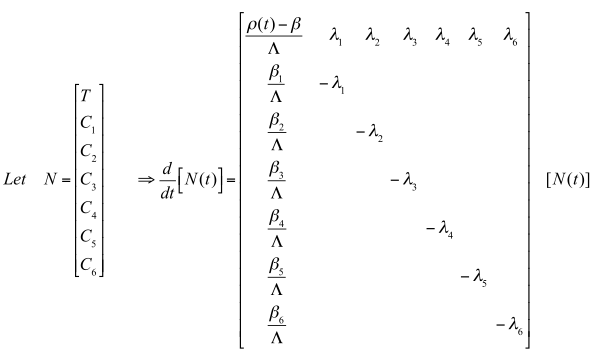
\includegraphics[width=4in]{images/pke/matrix-form.png}
%\end{figure}
\end{enumerate}

\clearpage
\topic{Application of PKEs}
\begin{enumerate}
\item Instantaneous reactor scram from criticality($\rho = - 8 \beta$). Power goes almost instantly to about 10\%, then it ultimately decays with time constant of longest lived precursor (55s in this case). 
  \begin{figure}[ht]
    \centering
    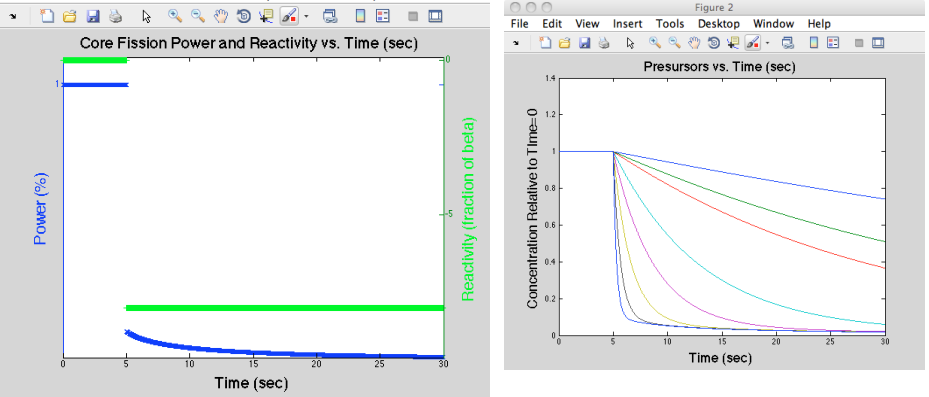
\includegraphics[width=5in]{images/pke/ex1.png}
    \caption{PKE Example 1, Instant Reactor Scram} 
  \end{figure}

\item 2s rod drop scram ($\rho = - 8 \beta$). Again, power goes to about 10\% when rod fully inserted, and power ultimately decays with time constant of the longest lived precursor (55s). 
  \begin{figure}[ht]
    \centering
    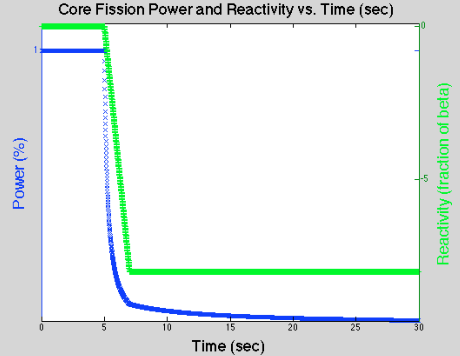
\includegraphics[width=3in]{images/pke/ex2.png}
    \caption{PKE Example 2, Two Second Reactor Scram} 
  \end{figure}

\clearpage
\item Instantaneous rod withdraw ($\rho = 0.1 \beta$). In this senario, there is only one delayed neutron precursor group, and we withdraw rod instantly. The reactor wants to response immediately (hence the jump) but it does not have enough delayed neutron to sustain that increase, hence the jump is not enough and it will increase for the rest of the way, until ultimately power increases with time constant of the longest precursor group (55s). See next section for the derivation of prompt jump estimation. 
  \begin{figure}[ht]
    \centering
    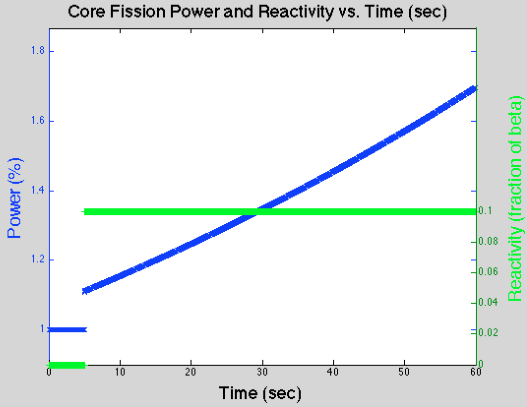
\includegraphics[width=3.5in]{images/pke/ex3.png}
    \caption{PKE Example 3, Instant Rod Withdrawal}  \label{ex3}
  \end{figure}
 


\item Instantaneous rod withdraw with 8 delayed groups. The intial part of the transient is slightly more complicated in Fig.~\ref{4a} than 1-group case in Fig.~\ref{ex3}(single delayed group is very sensitive to the time-constant). Fig.~\ref{4b} shows that, if we wait long enough,  we reach secular equilibrium between power and precursor rate that the precursor rates have the same shapes as the power, altough the rates may be off by a factor. 
  \begin{figure}[ht]
    \begin{subfigure}[b]{0.45\textwidth}
      \centering
      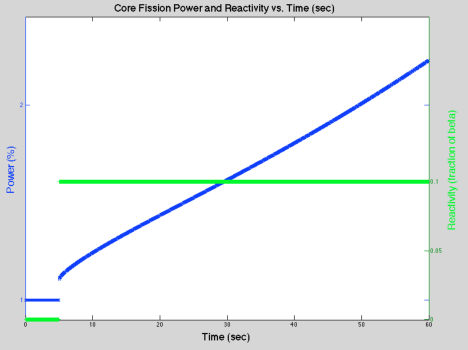
\includegraphics[width=\textwidth]{images/pke/ex4.png}
      \caption{Short Term Behavior} \label{4a} 
    \end{subfigure}
    \begin{subfigure}[b]{0.45\textwidth}
      \centering
      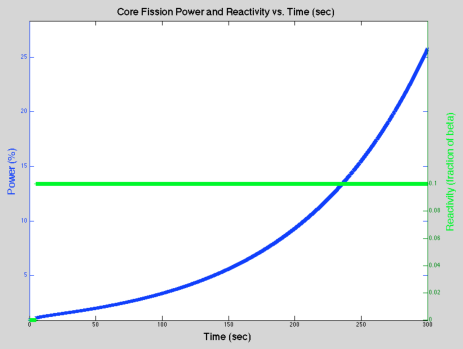
\includegraphics[width=\textwidth]{images/pke/ex4b.png}
      \caption{Long Term Behavior} \label{4b} 
    \end{subfigure}
    \caption{PKE Example 4, Instant Rod Withdrawal With 8 Delayed Groups} \label{ex4}
  \end{figure}

\item 2s rod insertion with 8 delayed groups ($\rho = -0.1 \beta$). 
  \begin{figure}[ht]
    \centering
    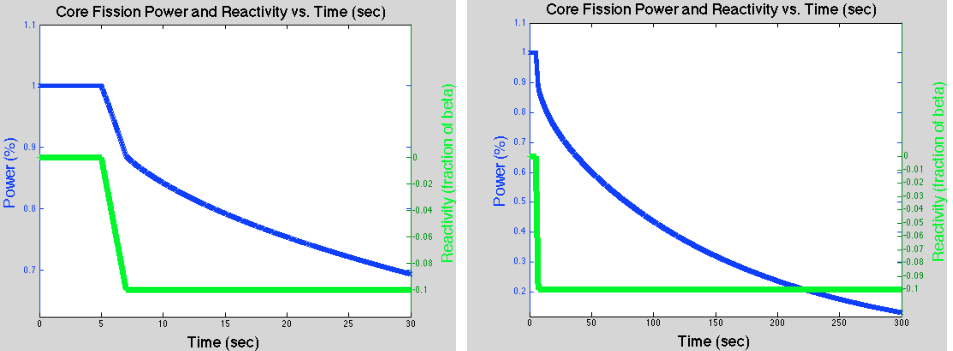
\includegraphics[width=6in]{images/pke/ex5.png}
    \caption{PKE Example 5, Two Second Rod Insertion} 
  \end{figure}

\item Regulating rod withdrawal/insertion. Senario: rod is moved in for 2s, hold for 20s, re-positioned in 2s. \textbf{Power does not come back to the original state, because we are solving for an eigenvalue problem, and what the asymptotic power is depends on how to get there.} In the withdrawal case, the precursor builds up and is continuing to build up during the second phase, so the power ends up higher than initially. 
  \begin{figure}[ht]
    \centering
    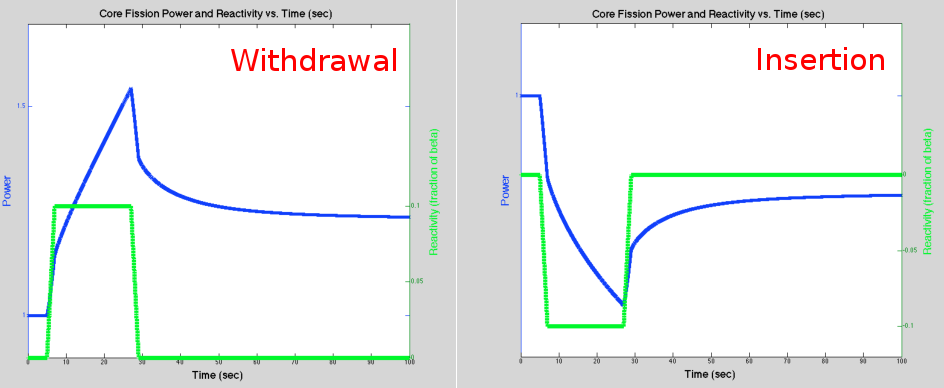
\includegraphics[width=6in]{images/pke/ex6.png}
    \caption{PKE Example 6, Rod Withdrawal and Insertion} 
  \end{figure}

\item Super-prompt criticality (failed housing). Senario: rod is moved in for 1s. The point is, power ascension is very sensitive as $\rho \approx \beta$. \textbf{When $\rho > \beta$, reactivity does not have to wait for the delayed neutrons anymore, changes can happen instantaneously.}
  \begin{figure}[ht]
    \centering
    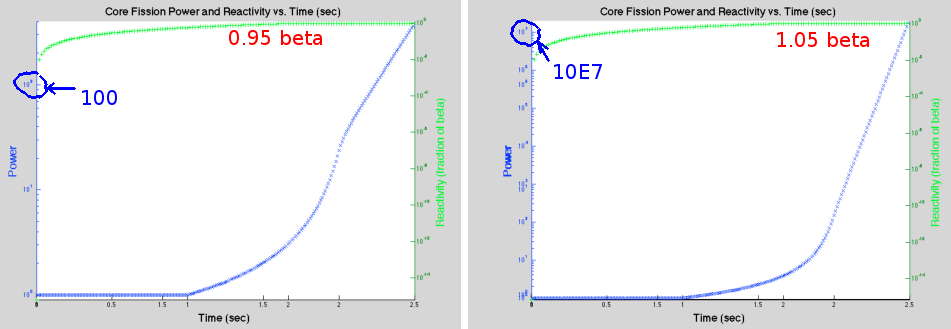
\includegraphics[width=6in]{images/pke/ex7.png}
    \caption{PKE Example 7, Failed Housing} 
  \end{figure}
  
\end{enumerate}



\clearpage
\topic{Inhour Equation}
\subtopic{Prompt-Jump Approximations}
To estimate the prompt jump, we do the prompt jump approximation (easy to do in 1 group). 
\begin{align}
\ddt T(t) &\approx 0 = \frac{\rho - \beta}{\Lambda} T(t) + \lambda C(t) \\
T(0^+) &= \frac{\Lambda \lambda}{\beta - \rho} C(0^+) = \frac{\Lambda \lambda}{\beta - \rho} \left[ \frac{\beta}{\Lambda \lambda} T_0 \right] \\
\Aboxed{ \frac{T(0^+)}{T_0} &= \frac{\beta}{\beta - \rho} }
\end{align}
Example: given a reactivity change of $0.1\beta$, the prompt jump is $\frac{T(0^+)}{T_0} = \frac{\beta}{\beta - 0.1 \beta} = 1.111$. 

\subtopic{In-hour Equations: The Simpliest Inverse Kinetics Application}
From the PKEs as in Eq.~\ref{in-hour}, we can derive the In-hour Equation. We assume the solution is in the form of,
\eqn{ T(t) &\approx C_i (t) \approx e^{\omega t}  }
Then $\ddt T(t) \approx \omega T(t), \ddt C_i(t) \approx \omega C_i(t)$, and hence PKEs in Eq.~\ref{in-hour} becomes, 
\eqn{ \omega T(t) &= \frac{\rho - \beta}{\Lambda} T(t) + \Sum_i \lambda_i C_i(t) \label{ih2} \\
  \omega C_i(t) &= \frac{\beta_i}{\Lambda} T(t) - \lambda_i C_i (t)  \label{ih3} }
From Eq.~\ref{ih3}, we can write $C_i(t)$ in terms of $T(t)$, 
\eqn{ C_i(t) = \frac{\beta_i}{\Lambda (\omega + \lambda_i)} T(t) }
Plug into Eq.~\ref{ih2}, 
\eqn{ \omega T(t) &= \frac{\rho - \beta}{\Lambda} T(t) + \Sum_i \frac{\lambda_i \beta_i}{\Lambda (\omega + \lambda_i)} T(t)  }
We cancel the $T(t)$ and multiply by $\Lambda$ on both sides,  
\eqn{ w \Lambda &= \rho - \beta + \Sum_i \frac{\lambda_i \beta_i}{\omega + \lambda_i} }
Recall that $\beta = \Sum_i \beta_i$, we can write the reactivity as, 
\eqn{ \rho = \omega \Lambda + \Sum_i \left( \beta_i - \frac{\lambda_i \beta_i}{\omega + \lambda_i} \right) }
That is, 
\eqn{ \Aboxed{ \rho &= \omega \Lambda + \Sum_i \frac{\beta_i \omega}{\omega + \lambda_i}} }
The point is, we can compute $\rho$ using inhour equation if we know $\beta_i, \omega, \lambda_i$. Another typically assumption is to set $\omega \Lambda \to 0$ because the prompt neutron lifetime is so small (with the exception of super prompt in which case $\omega$ is huge). The specific steps of computing $\rho$ for a reactor, 
\begin{enumerate}
\item Withdraw reactor control rod.
\item Measure reactivity period $T$ (make sure $T$ is constant before we measure it).
\item Use inhour equation to compute reactivity: $\omega = \frac{1}{T}$, plug $\omega$ into inhour equation. 
\end{enumerate}
This is how control rods are calibrated, and how small sample worths are measured. 

\subtopic{Reactivity Units}
\begin{table}[ht]
  \centering
  \begin{tabular}{|c|c|c|} \hline
    Unit & Definition & Example \\ \hline
    $\Delta k$ & actual units of PKEs & 0.01 \\
    \% $\Delta k$ & & 1\% \\
    pcm & $10^5 \Delta k $ & 1000 pcm \\ \hline
    Dollars & $\frac{\Delta k}{\beta}$ & \$1.5 \\
    Cents & 100 Dollars & 150 cents \\ 
    Milli-beta & 1000 Dollars & 1500 milli-beta \\ \hline
  \end{tabular}
  \caption{Common Reactivity Units}
\end{table}

\subtopic{Applications of Inhour: HZP Rod Worth Measurement}
Inhour equation can be used to measure HZP rod worth due to Boron dilution. The steps are: 
\begin{enumerate}
\item Make reactor stable (this is important, because without asymptotic period we cannot use the Inhour equation). 
\item Start Boron dilution. 
\item Move control rod in small number of steps and then wait.
\item Use point kinetics to convert ex-core detector signal into reactivity.
\item Infer differential and integral rod worths.
\end{enumerate}
Fig.~\ref{inhour-app} demonstrate this process. The problem is, the entire process takes more than 1 hour for each rod (because we have to carefully wait for the power to stablize after each step). This is too costly for real reactors, hence we need to derive a more general expression, which leads us to the next section on IK. 
\begin{figure}[ht]
  \centering
  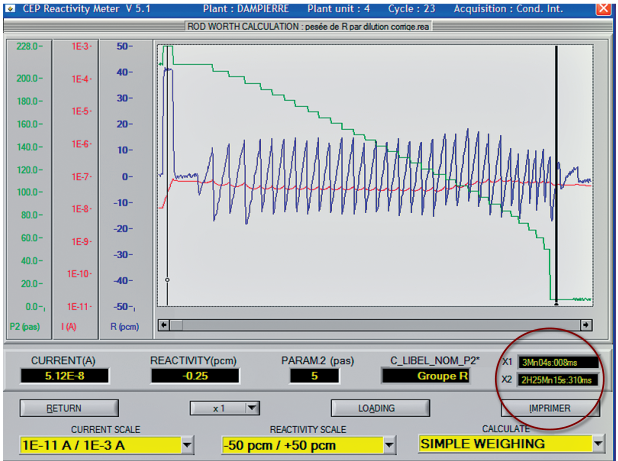
\includegraphics[width=4in]{images/pke/inhour-app.png}
  \caption{HZP Rod Worth Measurement: Boron Dilution}\label{inhour-app}
\end{figure}


\clearpage
\topic{Derivation of IK}
Assume we know the amplitude function $T(t)$ (that is, we are given a desired reactor power shape vs. time), we can solve for the pre-cursor function $C(t)$; then plugging back in the PKEs, we can get $\rho(t)$, that is, how to operator reactor to achieve the desired power shape. 
\begin{enumerate}
\item Given $T(t)$, we can solve for the precursor equations, 
\begin{align}
\ddt C_i(t) &= \frac{\beta_i}{\Lambda} T(t) - \lambda_i C(t) \\
\ddt C_i (t) + \lambda_i C_i(t) &= \frac{\beta_i}{\Lambda} T(t) 
\end{align}
If we define matrix $[A] = \mathrm{diag}[\lambda_i], [B] = \frac{\mathrm{diag}[\beta_i]}{\Lambda}, [Y(t)] = [B] T(t)$, then the above equation forms a matrix system for all $i$,
\eqn{ \ddt [C(t)] + [A] [C(t)] = [B] T(t) = [Y(t)] }

\item Multiply by IF $[e^{At}]$, 
\begin{align}
[e^{At}] \ddt[C(t)]  + [e^{At}][A] [C(t)] &= [e^{At}] [Y(t)] \\
\ddt \left( [e^{At}][C(t)]  \right) &=  [e^{At}] [Y(t)]
\end{align}

\item Integrating both side from $0$ to $t$, define $C_0 = C(t=0), Y_0 = Y(t=0)$,  
\eqn{ [e^{At}][C(t)] - [C_0] &=  [A]^{-1} \left( [e^{At}] [Y(t)] - [Y_0] \right)  }
\eqn{ \Aboxed{ [C(t)] &= [e^{-At}][C_0] + [e^{-At}] [A]^{-1} \left( [e^{At}][Y(t)] - [Y_0] \right) } }
where $[A] = \mathrm{diag}[\lambda_i], [Y(t)] = \frac{\mathrm{diag}[\beta_i]}{\Lambda} T(t)$.
That is, we can solve for the time-varying concentrations of precursors for any desired reactor power shape in time by applying this equation successively for discrete steps. 

\item From the PKEs, we can solve for the reactivity in terms of $C(t), T(t)$ by making finite-difference approximation for derivative term: 
\eqn{ \ddt T(t) &=  \frac{\rho(t) - \beta}{\Lambda} T(t) + \Sum_i \lambda_i C_i (t) + Q(t) }
\begin{align}
\Aboxed{\rho(t) &= \frac{\Lambda}{T(t)} \ddt T(t) + \beta - \frac{\Lambda}{T(t)} \Sum_i \lambda_i C_i(t) - \frac{\Lambda}{T(t)} Q(t) } \\
\Aboxed{ \rho_n &= \frac{\Lambda}{T_n} \frac{T_n - T_{n-1}}{t_n - t_{n-1}} + \beta - \frac{\Lambda}{T_n} \Sum_i \lambda_i C_{i,n} - \frac{\Lambda}{T_n} Q_n } 
\end{align}
\end{enumerate}


\clearpage
\topic{Applications of IK}
\subtopic{PWR Boration/Dilution}
\begin{figure}[ht]
  \centering
  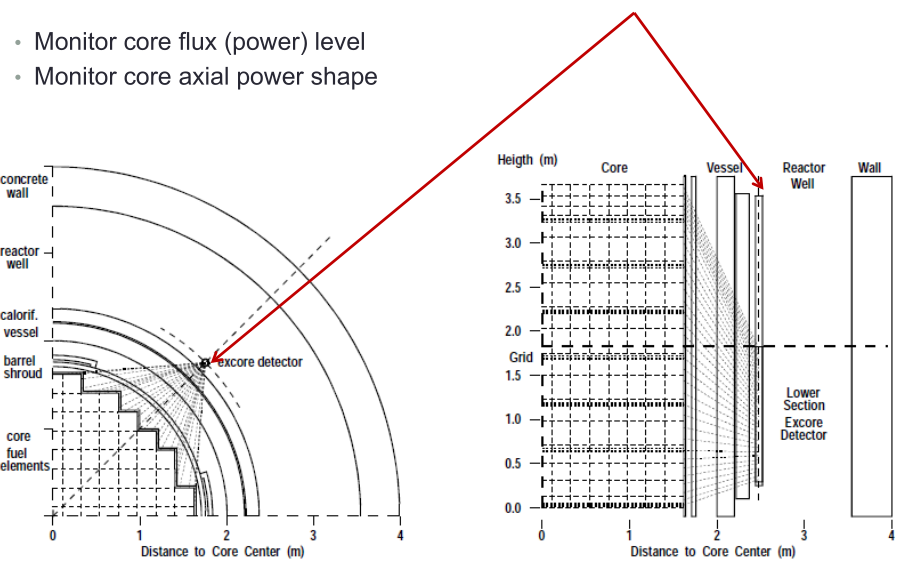
\includegraphics[width=4in]{images/pke/ik-ex1.png}
  \caption{IK Example 1, PWR Ex-core Detectors} \label{ik-ex1}
\end{figure}
The red lines in Fig.~\ref{ik-ex1} point out the location of the excore detectors. Prompt neutron life time is so short, so that even spatial distribution flux changes a lot, we can assume that it stabalizes already at each rod drop. 
\begin{itemize}
\item Disadvantages: time concern; boration dilution increases cost with waste disposal.  
\item Alternatives: we use General Inverse Kinetics to get around about it. 
\end{itemize}

\subtopic{SCRAM/Rod Drop Analysis}
  \begin{figure}[ht]
    \begin{subfigure}[b]{0.45\textwidth}
      \centering
      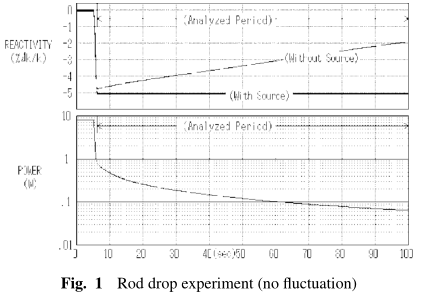
\includegraphics[width=\textwidth]{images/pke/ik-ex2a.png}      
      \caption{No Fluctuation} \label{ik-ex2a} 
    \end{subfigure}
    \begin{subfigure}[b]{0.45\textwidth}
      \centering
      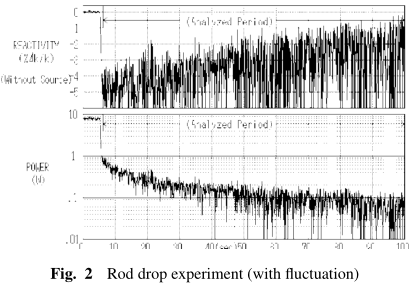
\includegraphics[width=\textwidth]{images/pke/ik-ex2b.png}      
      \caption{With Fluctuation} \label{ik-ex2b} 
    \end{subfigure}
    \caption{IK Example 2, Rod Drop for SCRAM Reactivity} \label{ik-ex2}
  \end{figure}
This example produces a scram, then measure power change and infer $T(t)$, thus estimate reactivity. The rough method use Prompt Jumpt Approximation. More accurately, we need to model all the neutron sources, including ($\alpha,n$) reactions etc.

In reality, there are noisy signals in measured power and reactivity data; we need to smooth them out with a fitted function before we can apply IK with external neutron sources. 

This technique is not used in the US that much because it is harsh your system and it requires work to bring the system back to critical. But it is one of the best ways to demonstrate to the licensing committee that a reactor is capable to scram.  

\subtopic{Dynamic Rod Worth}
We start with a critical reactor, and drive a control rod in and out and repeat with a different rod. The advantages are: no need to do boron dilution, and it takes 15 mins for each rod. This technique is widely used by Westinghouse to estimate their rod worth. 
\begin{figure}[ht]
  \centering
  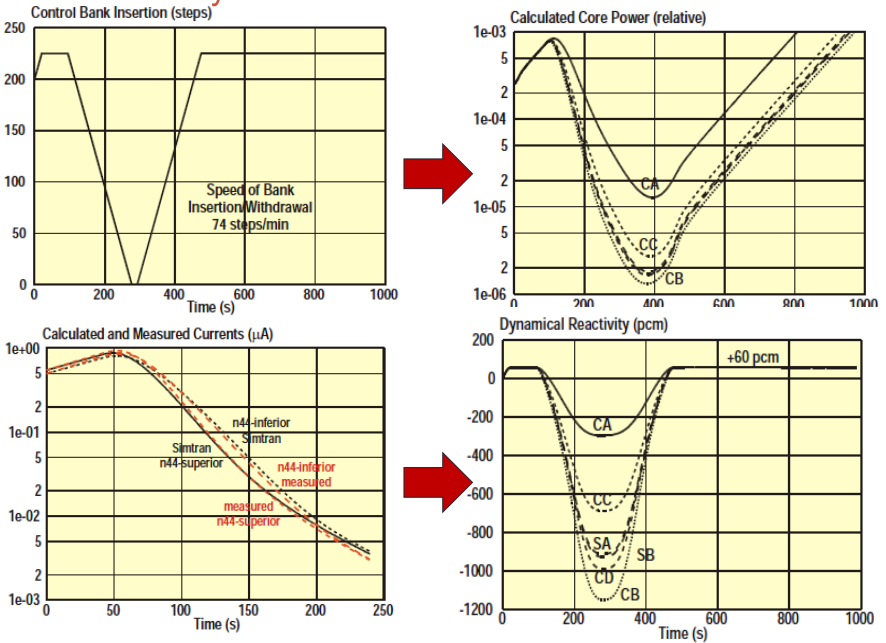
\includegraphics[width=4in]{images/pke/ik-ex3b.png}
  \caption{IK Example 3, PWR Dynamic Rod Worth} \label{ik-ex3}
\end{figure}

Alternatively, we can do sub-critical source multiplication, that is, IK with a source in the reactor. This way we don't even need to start with a critical reactor. This technique has only been used in experimental reactors but not so much in power reactors because it requires detailed knowledge about the source distribution. 

Note: we should be careful about power leve, as power can change from a few watts to 20,000 MW in less than a second! 
\begin{figure}[ht]
  \centering
  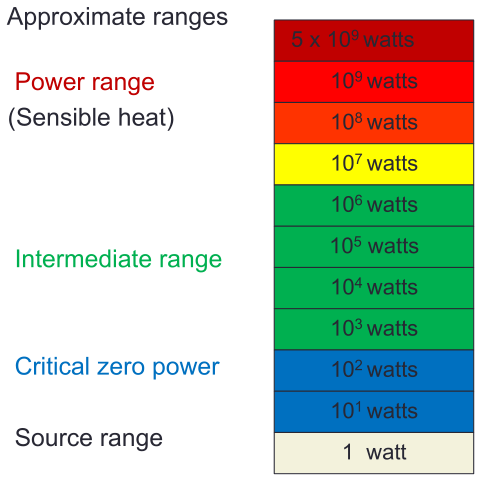
\includegraphics[width=4in]{images/pke/power-range.png}
  \caption{IK, Be Careful of Reactor Power Level} \label{power-range}
\end{figure}


\end{document}
